\chapter{Towards better understanding of relational latent representations}\label{ch:embeddinganalysis}


This chapter focuses on analysing the properties of relational latent representations.
It starts by analysing the representations created by CUR$^2$LED and identifies two properties -- entropy and sparsity, that offer insights into why representations created by CUR$^2$LED are effective.
The second contribution of this chapter is a systematic comparison of logic-based \gls{srl} and \gls{ilp} methods with knowledge graph embeddings on a set of standard benchmarks.



\section{Why are CUR$^2$LED representations effective?}

Latent features produced by \gls{curled} have proven useful in reducing the complexity of models and improving their performance.
However, no explanation was offered why that is the case.
In this section, we look into the properties of these latent representations and offer a partial explanation for their usefulness.
To answer this question we introduce the following properties: label entropy, sparsity and redundancy.



Label entropy and sparsity serve as a proxy to a quantification of learning difficulty -- i.e., how difficult is it to learn a definition of the target concept.
Considering a particular predicate, label entropy reflects a \textit{purity} of its true groundings with respect to the provided labels.
Intuitively, if true groundings of predicates tend to predominantly focus on one particular label, we expect model learning to be easier.


Sparse representations, one of the cornerstones of deep learning \cite{Bengio2013RLR}, refer to a notion in which concepts are explained based on local (instead of global) properties of instance space.
Even though many properties might exist for a particular problem, sparse representations describe instances using only a small subset of those properties. 
Intuitively, a concept spread across a small number of local regions is expected to be easier to capture than a concept spread globally over an entire instance space.



Quantifying sparsity in relational data is a challenging task which can be approached from multiple directions -- either by analysing the number of true groundings or interaction between entities, for instance.
We adopt a simple definition: the number of true groundings of a predicate.


Label entropy and sparsity jointly describe a compelling property of data representation --  instances space is divided in many local regions that match labels well  and consequently make learning substantially easier.



\textbf{Redundancy.} 
A downside of CUR$^2$LED is the high number of  created features. 
Despite their proven usefulness, a high number of latent features enlarges the search space of a relational model and increases the difficulty of learning.
As similarity interpretations are provided by the user, it is possible that almost identical clusterings are obtained with different similarity interpretations.
Thus, if many of the features are redundant, removing them simplifies learning.

We measure the redundancy with the \textit{adjusted Rand index} (ARI) \cite{Rand71,MoreyARI}, a standard measure for overlap between clusterings, and study its impact on the performance.
To evaluate the influence of redundant features, we modify CUR$^2$LED by adding an additional \textit{overlap parameter} $\alpha$.
Every time a new clustering is obtained, we check its overlap with the previously discovered clusterings using the ARI.
If the calculated value is bigger than $\alpha$, the clustering is rejected.



\subsection{Experiments and results}

We devise the experiments to answer the following questions:
\begin{itemize}
    \item[\textbf{(Q1)}] \textit{Do latent features that result in models of lower complexity and/or improved performance exhibit a lower label entropy compared to the original data representation?}
    \item[\textbf{(Q2)}] \textit{Are latent representation that improve the performance of a model sparser than the original data representations?}
    \item[\textbf{(Q3)}] \textit{To which extent are latent features redundant?}
\end{itemize}

\subsubsection{Datasets and setup}

The results  obtained in \cite{Dumancic2017} can be divided in three categories.
The first category contains the IMDB and UWCSE datasets; these datasets present easy relational learning tasks in which the original data representation is sufficient for almost perfect performance.
The main benefit of latent representations for these tasks was the reduction of model complexity.
The second category includes the TerroristAttack dataset, in which the main benefit of latent representation was the reduction of complexity, but not the performance.
The third category involves the Hepatitis, Mutagenesis and WebKB datasets.
These tasks benefited from latent representations in both performance and reduced model complexity.
That is especially true for the Hepatitis and WebKB datasets on which the performance was improved by a large margin.


We take a representative task from each of the categories.
Precisely, we use IMDB, UWCSE, Hepatitis and TerroristAttack datasets in our experiments.
Both IMDB and UWCSE datasets were included as they are easy to understand without the domain knowledge, and thus useful for analysing the interpretability of relational latent features.
As for the parameters of latent representation, we take the best parameters on individual datasets selected by the model selection procedure in \cite{Dumancic2017}.
When analysing the interpretability, we set $\theta$ to $0.3$.

When evaluating the redundancy, we create latent representations by setting the $\alpha$ to the following values: $\{0.9, 0.8, 0.7, 0.6, 0.5\}$.
We then learn a relational decision tree TILDE \cite{Blockeel1998285} on the obtained representation and compare accuracies, the number of created features and the number of facts.


When analysing the entropy and sparsity of representations, predicates indicating labels (such as \texttt{Professor} or \texttt{Student}) and entity definitions (such as \texttt{Person} or \texttt{Course}) are not considered in the analysis.


\subsubsection{Results}


\begin{figure}[t]
	\centering
	\medskip
    \includegraphics[width=1\textwidth]{entropy}
    \caption{Latent representations for IMDB, UWCSE and Hepatitis datasets contain substantially larger number of predicates (and the corresponding facts) with low label entropy, compared to the original representation of data. On the TerroristAttack dataset, for which the latent representation has not been useful, that is not the case - both original and latent representation demonstrate similar trends in label entropy of the predicates and the corresponding facts.}
    \label{fig:Entropy}
\end{figure}


\textbf{Label entropy.}
Figure~\ref{fig:Entropy} summarizes the label entropy for each dataset.
In all cases where representation learning proved helpful (i.e., IMDB, UWCSE, Hepatitis), latent representations have a substantially larger number of predicates with low label entropy compared to the original data representation. 
The latent representation for the TerroristAttack datasets, however, shows a different behaviour in which latent features with high entropy dominate the representation.
These results agree with the expectation that a high number of low entropy features makes learning easier.
However, not all latent features have low label entropy.
This is expected, as the labels are not considered during learning of latent features.
It also does not pose a problem -- these latent features are less consistent with the one particular task, but it might well be the case that those features are useful for a different task.




\begin{figure}
	\centering
	\medskip
    \includegraphics[width=1\textwidth]{sparsity}
    \caption{Latent representation tends to be sparser than the original representation on the datasets where it is beneficial (IMDB, UWCSE and Hepatitis). On the TerroristAttack dataset, where the latent representation is not beneficial, both original and latent representation follow the same trend. }
    \label{fig:Sparsity}
\end{figure}


\textbf{Sparsity.}
Figure~\ref{fig:Sparsity} summarizes the sparsity results in terms of the number of true instantiations of predicates.
The distribution of the number of true groundings in the latent representations (where latent features are beneficial) is heavily skewed towards a small number of groundings, in contrast with the original representation.
That is especially the case with the Hepatitis dataset, which profits the most from the latent features.
The exception to this behaviour is again the TerroristAttack dataset in which the original representation already is very sparse.
These results indicates that latent features indeed describe smaller groups of instances and their local properties, instead of global properties of all instances. 





\begin{figure}
	\centering
	\medskip
    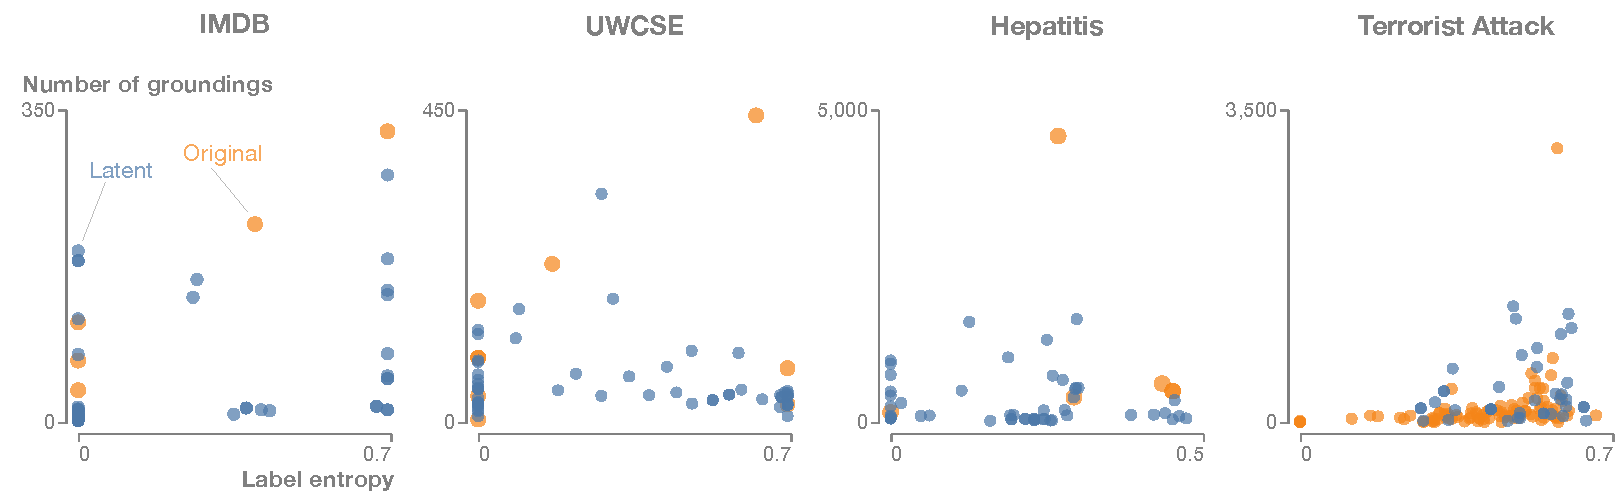
\includegraphics[width=1\textwidth]{combined}
    \caption{Contrasting the label entropy of predicates and the number of true groundings reveals that the many latent predicates with the low label entropy have similar number of groundings as the predicates of the original data representation. This means that the trivial case, in which a large number of low-entropy predicates is obtained due to many predicates that have just a few true groundings, is not explanation for the experimental results. Instead, the latent representation, when beneficial, successfully identifies local regions in the instance space that match well with the provided labels. The exception to this is again the TerroristAttack dataset.}
    \label{fig:EntropyVsSparsity}
\end{figure}




\textbf{Connecting label entropy and sparsity.}
A potential explanation of the above discussed results might be that many latent features capture a very small number of instances (e.g., 1 or 2) which would lead to a large number of features with low label entropy.
Such features would largely be useless as they make generalization very difficult.
To verify that this is not the case, Figure~\ref{fig:EntropyVsSparsity} plots the label entropy versus the number of groundings of a predicate.
If latent features of low label entropy would indeed capture only a small number of instances, many points would be condensed in the bottom left corner of the plot.
However, that is not the case -- many latent predicates with low label entropy actually have a number of groundings comparable to the predicates in the original representation.
The exception to this is again the TerroristAttacks dataset.

These results jointly point to the following conclusion: \textit{latent features successfully identify local regions in the instance space that match well with the provided labels}.
As a consequence, these local regions are easier to capture and represent.









\textbf{Redundancy.}
Figure~\ref{fig:Redundancy} summarizes the influence of $\alpha$ on the accuracy and the number of latent features.
The figure shows relative reduction in the number of features (equal to the number of predicates), the number of facts and the accuracy with  respect to the latent representation obtained without rejecting the overlapping clusterings.
These results show that the performance of the classifier is not affected by removing features based on the overlap of clusterings they define.
The performance of TILDE remains approximately the same, whereas the number of latent features is reduced by 20 to 30 \%.
As the number of features is directly related to the size of the search space of relational model (and thus the complexity of learning), this is an encouraging result indicating that the size of the search space can be naively reduced without sacrificing the performance.








\begin{figure}[t]
	\centering
	\medskip
    \includegraphics[width=1\textwidth]{redundancy_combined}
    \caption{The performance in terms of the accuracy is barely effected by removing overlapping clusterings, while the number of predicates and facts can be reduced up to 30\%. The only noticeable reduction in performance happen on the Hepatitis dataset, but only for approximately 5\%.   }
    \label{fig:Redundancy}
\end{figure}







\subsection{Looking forward}


The proposed experimental framework is only the first step towards understanding how latent representations can benefit relational learning methods.
The interaction between label entropy and sparsity seems to play an important role, indicative of the benefit of a latent representation.
On the other hand, the method for extracting the meaning of the latent features and analysis of their redundancy are developed especially for CUR$^2$LED and might have a limited benefit for future approaches.



Understanding when learning latent representation is (not) beneficial is an important question for further research.
Majority of tasks benefits from learning latent representations, but some, like the TerroristAttack dataset, do not.
Though we cannot definitely explain why that is the case, we suspect that the reason might be that the features of instances contain the most relevant information while the structure is uninformative.
In contrast, CUR$^2$LED is developed to exploit the rich structure in relational dataset and is thus not suited for the scenario where only the features are relevant.




Another important question is how this kind of insights connects to the embeddings to vector spaces.
The analysis done in this work focuses on contrasting the properties of predicates and associated data of original and latent representation obtained by CUR$^2$LED.
The embeddings to vector spaces replace the logical representation of data with points in the Euclidean space and are thus not amenable to this kind of analysis.
However, similar kind of analysis for embedding spaces is currently missing in the literature.
Further research towards combining relational and deep learning methods might greatly benefit from understanding up- and downsides of both directions of research, and developing new ideas that combine advantages of both.


\section{On embeddings as an alternative paradigm for relational learning}


%Learning from complex relational domains, where data contains instances and their mutual relationships, has typically been the focus of logic and graph-based machine learning methods.
%\textit{Statistical relational learning} (SRL)  \cite{Getoor:2007,Raedt:2016:SRA:3027718} uses the representational and reasoning framework of first-order logic to compactly represent such data, and combines it with probabilistic graphical models to facilitate reasoning under uncertainty.
%As first-order logic is a very general representation language, it serves as a unifying representational framework for many tasks such as classification, clustering, link prediction, and probabilistic modelling.
%\textit{Graph mining} (GM) approaches  \cite{Chakrabarti:2006:GML:1132952.1132954} approach relational data as graph-structured data.


\textit{Representation learning} for relational data has shown promising results for specific relational tasks such as knowledge base completion~\cite{Nickel0TG16}.
Knowledge graph embedding (KGE) methods take a radically different approach from the symbolic methods, and aim to represent instances and their relationship as vectors and/or matrices in the Euclidean space.
Intuitively, KGEs introduce a novel view on relational propositionalization \cite{Kramer2001}.
The hope is that the geometry of the embedding space would resemble the structure of the data by, for example, keeping the instances participating in the same relationships close in the Euclidean space.
This in turn allows one to apply standard propositional machine learning tools and retain their scalability, while at the same time preserving certain properties of structured relational data.
These methods have proven to be very effective for the task of knowledge graph completion, where the goal is to identify missing links in the existing knowledge graph. They have also proven to be scalable to very large knowledge graphs.


Motivated by the success of KGE methods, there has been some recent work on combining more traditional logic-based SRL with representation learning methods.
\cite{Sourek:2015:LRN:2996831.2996838}   introduce a relational extensions of neural networks (NN) by developing a template language for constructing neural networks from logical rules and data.
\cite{Kazemi2018} take a different view on relational NNs by means of the the relational logistic regression \cite{KazemiLR2014}.
\cite{Dumancic2017} introduced a task-agnostic relational latent feature learning pipeline based on clustering that can be combined with any relational learner.





Unfortunately, these research directions have largely been developed in isolation and little understanding is currently available on the relative advantages of the respective approaches.
Not only do they focus on different tasks but also different evaluation metrics.
\gls{kge} methods, also referred to as \textit{latent feature models}, typically focus on knowledge graph completion which requires very simple forms of relational reasoning. The evaluation metrics are often measuring the quality of rankings generated by the respective scoring functions. 
\gls{srl} methods, also referred to as \textit{observed feature models}, typically focus on learning from small relational data, employing more complex forms of logical reasoning.


The focus of these methods already outlines the basic understanding of their limitations.
A major advantage KGE methods is their scalability -- they easily operate on knowledge graphs with millions of facts and thousands of relations.
The main drawbacks of KGE methods are the black-box nature, limited reasoning on local information, and the difficulty of handling unseen instances.
\gls{srl} methods are capable of capturing very complex relational patterns, are interpretable, and generalize beyond seen data. Unfortunately, both inference and learning in SRL is highly complex, limiting its applicability.



In this work, we systematically compare KGE and logic-based SRL methods on standard relational classification and clustering tasks. We hope this contributes to a better understanding of their relative strengths and weaknesses. We focus on standard relational data sets as they offer more variety of tasks and reasoning complexity. We include both quantitative, in terms of performance, and qualitative analysis, in terms of extracted patterns of reasoning, in order to gain more insights into the suitability of these different methods. 
 








%%%%%%%%%%%%%%%%%%
%
%	RELATED WORK
%
%%%%%%%%%%%%%%%%%%
\subsection{What do we know so far?}

%\paragraph{Knowledge graph embeddings}

%Knowledge graph embeddings have emerged as an alternative paradigm for learning and reasoning with structured relational data.
%They replace symbols, i.e. instances and their relation predicates, with vectors and matrices in Euclidean space.
%That way the reasoning is performed through algebraic manipulations instead of more costly logical inference.
%The underlying idea of KGE methods is to associate a score with atoms in a database.
%Learning then consists of finding the vector representation of instances and their relations by maximizing (minimizing) the scores of the atoms in the database and minimizing (maximizing) the score of atoms not in the database.
%Two prototypical examples are:
%\begin{itemize}
	%\setlength{\itemindent}{1.2cm}
%	\item \textbf{TransE} \cite{BordesNIPS2013} which interprets relations as translations between instances in the Euclidean space. For each atom \texttt{r(h,t)}, \texttt{r} being a relation and \texttt{h} and \texttt{t} \textit{head} and \textit{tail} instances respectively, the score equals
 % 				$$ s(r,h,t) = -||\mathbf{e}_h + \mathbf{e}_r - \mathbf{e}_t ||, $$
 % 				i.e., the vector representation $\mathbf{e}_h$ of a \textit{head} instance translated by the relation vector $\mathbf{e}_r$ should be close to the vector representation $\mathbf{e}_t$ \textit{tail} instance
%	\item \textbf{DistMult}  \cite{YangYHGD14a} which focuses on pairwise interactions of \textit{latent} features with the following score
%				$$ s(r,h,t) = (\mathbf{e}_h \ocircle \mathbf{e}_r)\mathbf{e}_t^T $$
%				where $\ocircle$ is an element-wise product.
%\end{itemize}

%Checking the validity/truthfulness of any fact comes down to evaluating its score. The majority of KGE methods proposed so far \cite{EmbeddingsOverview} are a variation on the above scoring functions.
 




Understanding of advantages and disadvantages of KGE and logic-based SRL methods is currently very limited.
\cite{NickleNIPS2014} show that including both observable patterns, in form of random walks over a knowledge graph, and latent features from KGEs can greatly increase their performance and reduce the learning complexity.
\cite{pujara:emnlp17} show that KGEs have difficulties handling data with high degree of sparsity and noise -- which is the case with every automatically created knowledge graph.  
Finally, \cite{VigILP2017} show that KGE could be beneficial when the background knowledge about the task at hand is limited, but if such knowledge is available then the SRL methods are preferable.
\cite{GrefenstetteTFDS}  introduces a formal framework for simulating logical reasoning through tensor calculation.












%%%%%%%%%%%%%%%%%%
%
%	METHODOLOGY
%
%%%%%%%%%%%%%%%%%
\subsection{Methodology}

The main goal of this study is to identify the strengths and weaknesses of  KGE and logic-based SRL approaches to learning and reasoning with relational data.
Concretely, we focus on the following questions:
\begin{itemize}
	\setlength{\itemindent}{1em}
	\item[\textbf{Q1}] \textit{Are KGEs a viable alternative to logic-based methods for relational classification?}
	\item[\textbf{Q2}] \textit{Are KGEs a viable alternative for relational clustering methods?} 
\end{itemize}

More specifically, we focus on the following tasks:
\begin{itemize}
    \setlength{\itemindent}{1em}
    \item[\textbf{T1}] Given a set of \textit{target instances} (entities in a knowledge base), learn a model that predicts the value of the labels associated with those instances. We consider fully relational models learning the logical theory for predicting the labels, and a feature based models learning from the vector representation of target instances.
    \item[\textbf{T2}] Given a set of instances of a specific type or domain, group them into a pre-specified number of groups. We consider methods operating on logical representation of data as well as those operating on the vector representation of instances.
\end{itemize}

Furthermore, we compare the two approaches across various tasks in order to \textit{determine under which conditions KGEs are preferable to logic-based SRL methods and vice versa}.
Given that KGEs are sensitive to the hyper-parameters, especially the size of the embeddings, we investigate the magnitude of those effects.
Sensitivity to the hyper-parameter setup is less of a concern for classification tasks where one can use labels to tune the hyper-parameters. However, it poses a major issue for clustering tasks where no labels exists and there are no clear-cut performance criteria.
A potential option would be to rely on certain geometric measures. These are, however, often based on various assumptions of limited generality and do not offer a performance measure such as classification accuracy~\cite{Estivill-Castro:2002}.


\begin{table}[t]
	\centering
	
	\caption{Dataset properties summarize the number of target and all instances, the number of attributes, and the number of relation types.}
	\begin{tabular}{@{}lcccccc@{}}
		\toprule
		\textbf{Dataset} 	& \multicolumn{2}{c}{\textbf{Instances}} 		& \multicolumn{2}{c}{\textbf{Attributes}}	& \multicolumn{2}{c}{\textbf{Relations}} \\
							\cmidrule(rl){2-3} \cmidrule(lr){4-5} \cmidrule(l){6-7}
							& Target 				& Total					&   Target				& Total				& Target		& Total						\\
		\midrule
		Hepa				& 500					& 5919					& 2						& 12				& 3				& 3						\\
		Muta				& 230					& 6124					& 3						& 7					& 3				& 7in						\\
		Terror				& 1293					& 1293					& 104					& 104				& 2				& 2						\\
		WebKB				& 920					& 3880					& 763					& 1207				& 4				& 5						\\
		\bottomrule
	\end{tabular}
	\label{tab:properties}
\end{table}


\paragraph{Data}
We take standard relational learning data sets and use the available labels as ground truth for both classification and clustering.
The IMDB data set is a snapshot of the Internet Movie Database, describing a set of movies with their actors and directors. 
The task is to distinguish between actors and directors.
The UWCSE data set describes the employees of the University of Washington, their roles, publications, and courses.
The task is to distinguish between students and professors.
The Mutagenesis data set consists of a set of molecules and their structures, with the goal of predicting whether a compound is mutagenic or not.
The WebKB dataset describes web pages of four US universities and their corresponding link structure.
The pages are classified into seven groups according to their roles such as personal, departmental or project page.
The Terrorists data set contains a network of terrorist attacks, each assigned to of the 6 types of attacks.
Finally, the Hepatitis data set describes a set of patients with a diagnosis of Hepatitis B and C.
We intentionally focus on standard relational learning data sets because they typically expose more variety of reasoning: required reasoning ranges from attribute-only reasoning to multi-hop reasoning.
Some of the properties are list in Table~\ref{tab:properties}.
For each property, we differentiate between target instances -- instances which contain labels, and the rest.
This gives us a better opportunity to detect the conditions under which either of the respective approaches is preferable.
In contrast, standard KB completion data sets are often very simple and  only simple path-type rules are required to achieve a reasonable performance.
Therefore, the only disadvantage of standard relational methods is that they might very inefficient because of the data set size.



\paragraph{Classification Experiments}
We perform standard nested cross-validation. For each split the training data is used to learn the models and tune their parameters (using an inner cross-validation loop) and the unseen fold is used for testing.
We report the performance in terms of accuracy as an average over individual splits. The labels were excluded from the data when learning the KGEs and considered only during the training of the classifier.


\paragraph{Clustering Experiments}
For the clustering experiments, we cluster the entire data set at once using the number of distinct labels as the number of clusters.
Once the clustering is obtained, we compare it to the ground truth determined by the class labels using the adjusted Rand index \cite{MoreyARI} as evaluation measure.
We use Spectral \cite{Spectral} and Hierarchical \cite{Agglomerative} clustering algorithms and compare embedding-based clustering with state-of-the-art relational clustering method ReCeNT \cite{Dumancic2017a}.
ReCeNT defines a very flexible similarity measure for relational objects which is used in the conjunction with the 


\paragraph{Knowledge Graph Embeddings}

Many KGEs exist in the literature \cite{EmbeddingsOverview}.
We decide to focus on two prototypical and commonly used instances: TransE  and DistMult. We evaluate the dimensions in $\{10, 20, 30, 50, 80, 100\}$ and train for 100 epochs.

As KGE methods are focused on the knowledge graph completion task, they assume that all instances are given at once and focus on filling in the missing links in data.
Therefore, they have difficulties with unseen instances.
We do not address this issue here, but simply learn the representation of both training and test data at the same time (with labels excluded).

\paragraph{Relational Learning}

We currently limit the analysis to Inductive logic programming (ILP) methods \cite{LucRLbook} and ignore the probabilistic aspect of SRL methods.
This is solely due to better predictive rule induction support of ILP.
For that reason, we decide to use the relational decision tree learner TILDE \cite{Blockeel1998285} as a relational  baseline.
We report results of two TILDE variants: one trained on the original (logical) data representation (termed TILDE), and the one trained on the \textit{relational} latent features created by CUR$^2$LED \cite{Dumancic2017} (termed TILDE-latent).
CUR$^2$LED creates latent features that remain in the logical representation (i.e., are expressed through predicate logic) and should not be confused with the vector representation based latent features.









\subsection{Classification Results}


\begin{figure}
	\centering
		\includegraphics[height=8cm]{classification.pdf}
		\caption{Classification performance. Individual rows contain results with distinct KGE methods. The color indicates whether the learning is propositional or relational. The performance of TILDE variants is simply duplicated on two graphs, for easier comparison.}
		\label{fig:classification} 
\end{figure}
		

\begin{figure}
	\centering
		\includegraphics[height=8cm]{classification_dimension}
		\caption{Performance of KGEs varies substantially with the dimension. The rows show performance of the KGE methods, while the brightness indicates the dimension. (WebKB has a separate scale because the performance is in a very different range compared to other datasets)}
		\label{fig:clasVariance}
\end{figure}
		





\begin{table*}[h!]
	\centering
	
	\caption{Properties of extracted rules are summarized as a proportion of relation and attribute predicates they contain. \textit{Rule properties} section describes the proportion of rules that contain  \textit{relation} predicates only, \textit{attribute} predicates only and the mix of both, for each dataset. \textit{Dataset properties} section shows the proportion of possible attribute and relation predicates that are used in the extracted rules. For example, the rules on the Hepatitis dataset use 100 \% of the possible attribute predicates, and 66 \% of relation predicates. \textit{Neighbourhood} refers to the proportion of attribute and relation predicates of the non-target instances for which a direct link with target instances exists. }
	\begin{tabular}{@{}lccccccc@{}}
		\toprule
		\textbf{Dataset}		& \textbf{Reasoning depth} 	& \multicolumn{3}{c}{\textbf{Rule properties}} 	& \multicolumn{3}{c}{\textbf{Dataset properties}} \\
		\cmidrule(lr){3-5} \cmidrule(l){6-8}
							& 				  			& Relations   		& Attributes 	& Mix		& Attributes        & Relations	& Neighbourhood	     \\
							\midrule 
		Hepatitis   		& 1.4				  		& 10 \%				& 38 \%			& 52 \%		& 100 \%					&  66 \%				& 70 \%				\\
		Terrorists			& 1							& 0	\%				& 95 \%			& 5 \%		& 35 \%				& 100 \%		& 0 \%			\\
		Mutagenesis			& 0							& 0 \%				& 100 \%		& 0 \%		& 100 \%					& 0 \%	& 0 \%				\\
		WebKB				& 2							& 5 \%				& 76 \%			& 19 \%		& 4 \%				& 50 \%		& 1 \%		\\ 	\bottomrule 	
	\end{tabular}
	\label{tab:ruleproperties}
\end{table*}


We first focus on comparing the classifiers with the same learning bias, namely propositional and relational decision trees (DT), as this constitutes the fairest comparison.
The results (Figure~\ref{fig:classification}) show that the decision tree trained on the embedding features outperforms TILDE only on the Hepatitis data set.
However, it does not outperform TILDE-latent on any data set. The performance is similar only on the Terrorists data set.
This implicates that relational learners are able to capture certain information that embeddings likely do not contain.
Moreover, fully acknowledging relational information (especially distinguishing between attributes of instances and their mutual relationships) while learning the latent representation \cite{Dumancic2017} seems beneficial as TILDE-latent outperform TILDE in all but one case.
An important aspect to keep in mind is that KGE methods see both training and test data at training time.
This gives them a certain advantage and the question is to what extent this effects the performance.
We did not observe significant difference between TransE and DistMult.


The classifiers with non-linear decision function, non-linear SVM and kNN, perform substantially better than the decision tree with the embedding features.
Even though both SVM and kNN are able to capture more complex feature interactions than a decision tree, the results indicate that their results are not significantly better than those of the relational methods.
SVM strongly outperforms TILDE on the Hepatitis dataset, both are similar in performance of the Mutagenesis and Terrorists dataset while TILDE performs much better on the WebKB dataset.
kNN slightly outperforms TILDE on the Hepatitis, performs slightly worse than TILDE on Mutagenesis and Terrorists, and substantially worse on the WebKB data set.
TILDE-latent outperforms SVM and kNN on the Mutagenesis and WebKB data, is much closer in performance to SVM and kNN of the Hepatititis but struggles with the Terrorists.
These results suggest that the ability to capture more complex dependencies allows SVM and kNN to compensate for the lack of the explicit relational information.
This also suggests that then labelled instance are not linearly separable in the embedding space, which explain why both SVM and kNN perform much better than DTs.




Analyzing these results with respect to the semantics of the predicates used in the extracted rules yields further interesting results.
More precisely, we differentiate between \textit{attribute predicates} that associate a specific value of an attribute with an instance, and \textit{relation predicates} that connect two instances.
We further distinguish between \textit{target} instances having an associated label, and \textit{neighbourhood} instances that provide additional data.
%We summarise (Table~\ref{tab:properties}) the properties of the rules induced by TILDE in terms of (i) \textit{the proportion of rules that are composed of relation predicates only, attributes predicates only and the mixture of both}, and (ii) \textit{the proportion of attribute and relation predicates used in the induced rules w.r.t. the available predicates in the dataset}.
Properties of rules learned by TILDE (Table~\ref{tab:ruleproperties}) suggest that KGE have an edge over the SRL methods when most of the information in the neighbourhood of instances is relevant.
For example, on the Hepatitis data set  the induced rules incorporate 100 \% of the target attributes and 66 \% of relations involving target instances, as well as 70 \% of the predicates related to the neighbouring instances.
This also holds for the Terrorists data; though 35 \% does not constitutes 'most of the information in the neighbourhood', we have found that many of the attributes are highly correlated and thus the number of predictive attributes is effectively higher.


The remaining two data sets are different in the sense that only a fraction of information is found predictive.
On the Mutagenesis data set\footnote{we use the version of the data set without any rings structures and additional background knowledge which is difficult to incorporate in KGE methods}, even though all the attributes of molecules are found predictive, none of the relations were found predictive and thus none of the information about atoms they contain.
Thus, only a fraction of available information is used.
On the WebKB data set only 4 \% of the attributes have been found predictive, as well as 50 \% of relations.
An explanation for such a big difference in performance might be that SRL methods have to select few predictive rules while learning theories, and thus can discard irrelevant information.
In contrast, the learning principle of KGEs is designed to take all of the information into account, which seems to make them underperform.



Figure~\ref{fig:clasVariance} show the differences in performances when the dimension of the embeddings is changed.
These results indicate the importance of choosing the embedding dimension, as the performance varies substantially with the dimension.
That is especially true for the Mutagenesis and WebKB datasets.
Unfortunately, there does not seem to be a general rules how to choose the dimension: higher does not lead to better results.
Fortunately, this is not a major issue for the classification tasks as the dimension can be treated as a parameter to tune.






\subsection{Clustering results}

The first issue when using KGEs for entity clustering is which distance or similarity measure to use.
Even though KGEs embed instances in Euclidean space, that space is usually high-dimensional and, thus, simple Euclidean distance is likely not to be informative.
Therefore, to better understand how to use KGEs for clustering, we first survey the possible distance and similarity measures.
We focus on the measure available in the \texttt{sci-kit learn} package \cite{scikit-learn} in combination with Spectral and Hierarchical clustering.



\begin{table}
	\caption{Ranking of similarity measure for Spectral clustering.}
		\label{tab:ranksSpectral}
		\begin{tabular}{@{}llcccccc@{}}
				\toprule
				\textbf{Embed}		& \textbf{Measure}	& \multicolumn{5}{c}{\textbf{Dimension}}	& \textbf{Avg} \\
								\cmidrule(lr){3-7}
								&					&  10	& 30		& 50	& 80 	& 100		&				\\
								\midrule
				transE			& polynomial			& 2.2	& 2.4	& 2.2	& 2.0	& 2.2		& 2.23			\\
								& sigmoid			& 2.8	& 3.6	& 3.2	& 2.4	& 3.2		& 3.0    \\
								& rbf				& 3.0	& 2.6	& 3.6	& 3.2	& 3.0		& 3.03		\\
								& laplace			& 4.0	& 3.0	& 3.3	& 3.4	& 3.4		& 3.33			\\
								& NN				& 3.0	& 3.8	& 3.6	& 3.2	& 3.6		& 3.4		\\
				distMult			& polynomial			& 3.2	& 1.6	& 1.6	& 1.6	& 1.4		& 1.9		\\
								& rbf				& 2.4	& 2.8	& 3.2	& 3.0	& 3.6		& 2.83        \\
								& sigmoid			& 2.6	& 3.0	& 2.6	& 2.4	& 2.8		& 2.9			\\
								& NN				& 3.6	& 3.4	& 3.8	& 3.4	& 3.0		& 3.53				\\
								& laplacian			& 3.2	& 4.2	& 3.8	& 4.6	& 4.2		& 3.83				\\
				\bottomrule	
				
			\end{tabular}
\end{table}
	
		
\begin{table}
	\caption{Rankings of distances for Hierarchical clustering.}
		\label{tab:ranksHierarchical}
		\begin{tabular}{@{}llcccccc@{}}
				\toprule
				\textbf{Embed}		& \textbf{Measure}	& \multicolumn{5}{c}{\textbf{Dimension}}	& \textbf{Avg} \\
								\cmidrule(lr){3-7}
								&					&  10	& 30		& 50	& 80 	& 100		&				\\
								\midrule
				transE			& cosine				& 3.8	& 6.0	& 3.8	& 3.8	& 4.4		& 4.43			\\
								& correlation		& 6.8	& 4.2	& 8.4	& 4.2	& 4.0		& 5.5    \\
								& braycurtis			& 8.4	& 5.2	& 4.6	& 4.2	& 8.4		& 6.37		\\
								& canberra			& 7.2	& 9.2	& 9.4	& 5.2	& 5.2		& 7.9			\\
								& chebysev			& 6.0	& 13.0	& 13.2	& 9.8	& 10.0		& 9.73		\\
				distMult			& correlation		& 6.0	& 3.8	& 8.0	& 2.0	& 7.4		& 5.87				\\
								& cosine				& 8.8	& 8.0	& 2.2	& 5.4	& 8.2		& 6.7        \\
								& braycurtis			& 7.2	& 8.8	& 5.8	& 2.6	& 5.8		& 6.83			\\
								& l1				& 6.2	& 7.4	& 9.2	& 11.8	& 7.2		& 8.0			\\
								& canberra			& 11.0	& 10.6	& 5.6	& 4.2	& 6.2		& 8.27				\\
				\bottomrule	
				
			\end{tabular}
\end{table}	
		
	




We first use every distance and similarity measure available to perform clustering for each of the dimensions in $\{10, 30, 50, 80, 100\}$.
Within each dimension, we rank the measure according to their performance per dataset and report average rank per dimension.
The ranks for the five best performing ones are reported in Table~\ref{tab:ranksSpectral} for Spectral clustering and in Table~\ref{tab:ranksHierarchical} for Hierarchical clustering.



These results suggest that clustering with KGE is not straightforward as there is no single measure that is an obvious winner.
Polynomial kernel seems to be the overall winner with spectral clustering, but it is mostly the second best measure to use on the individual data set.
The results with hierarchical clustering show even greater variance: cosine and correlation distances seem to be an overall winner but they average ranks spread between 4 and 6.
This means that a different distance/similarity measure is the most appropriate one for each data set, but at the same time it performs bad with different data set and embeddings dimension,
Therefore, a major challenge with using KGEs as a means for relational clustering is the choice of the right distance or similarity, but unfortunately clustering settings does not provide a ground truth that can be used to find the most suitable measure.
In further experiments, we use cosine and polynomial distance.


\begin{figure}
	\centering
	\includegraphics[width=.8\linewidth]{clustering}
	\caption{Clustering performance per dataset. The first two rows correspond to distinct KGE methods, while the third one contains results of the relational clustering approach.  }
	\label{fig:clustering}
\end{figure}


Comparing the performance of clustering approaches yields mixed results (Figure~\ref{fig:clustering}).
For instance, on the IMDB data set embeddings do better than the relational methods with Hierarchical clustering, while the relational methods substantially outperforms KGEs with Spectral clustering.
Similar holds for the Terrorists and WebKB data.
However, on the Mutagenesis and UWCSE data sets, relational methods to better in both cases.
With an exception in the Terrorists data, the best overall result is achieved by the relational learning approach.
It is interesting to note that these are the same data sets where relational methods have the advantage in the classification settings.
It is also interesting to note that, while relational clustering method seems to achieve better results with Spectral clustering, the performance of clustering algorithms is more balanced in the case of KGEs.
This implies that the KGEs introduce \textit{smoother} geometry that is more accessible to wider class of clustering algorithms, but more elaborate experiments are needed to confirm this.






\begin{figure}
	\centering
	\includegraphics[width=.8\linewidth]{clustering_dimension}
	\caption{The performance of clustering method varies substantially with dimension (indicated by the brightness). }
	\label{fig:clusVariance}
\end{figure}



Unfortunately, using KGEs for clustering seems to be highly sensitive to the choice of dimension (Figure~\ref{fig:clusVariance}).
Simply altering the dimension varies the results from a completely random clustering (ARI$\approx 0$), to the best obtained one.
As finding the means to somehow choose the correct value directly from the data is very difficult for clustering, this severely limits the applicability of KGEs for clustering tasks.



\subsection{Conclusions and Future Work}


The most important takeaway messages from this work are the following:
\begin{itemize}
	\item \textbf{KGE seems to be suitable for curated data} KGEs seem to have difficulties in the case when only a small fraction of available information is necessary for the given prediction task. SRL methods do not have that issue as they cherry pick useful information during the learning phase. This observation explains why KGEs perform well on the knowledge base completion task where the complexity of reasoning is low, but the dataset is huge. This further indicates the target use cases for the respective approaches: KGEs target simple relational reasoning with huge amounts of data, while SRL targets complex reasoning tasks with not a lot of data.
	\item \textbf{KGE might be useful for relational clustering but needs further research} Although logic-based relational clustering algorithms achieve the overall best results, clustering instances in the embeddings space does not lack much behind. They certainly show potential for this task, however they rise many problem, such as the question of an appropriate distance/similarity measure.
	\item \textbf{Hyper-parameters matter a lot} A major disadvantage of KGEs is their sensitivity to hyper-parameters. Out experiments show there is no clear strategy for choosing the right dimension. Though this might be less of an issue for classification problems, it poses a major one for clustering where there is no option to tune the parameters.
\end{itemize}


Besides the above outlined point, some obvious (dis)advantages are worth re-iterating here.
A strong advantage of KGEs is their scalability, at the expense of their black-box nature and limited reasoning capabilities.
SRL methods are a direct opposite -- they can capture very complex reasoning, are interpretable but currently of a limited scalability.



The analysis presented here is still preliminary and has to be extended in several ways.
We plan to extend this study in three main directions.
First, adding more datasets is necessary to confirm the preliminary results.
Second, including a larger variety of relational learners is necessary to get a complete picture.
Currently we considered only TILDE as the relational baseline, which was often outperformed by SVM and kNN trained on the embeddings of entities.
Therefore, a fairer comparison would be to compare embedding-based SVM and kNN with relational learners with similar non-linear decision functions such as kFOIL \cite{Landwehr:2006:KLS:1597538.1597601}, nFOIL \cite{Landwehr:2005:NIN:1619410.1619460} and kNN with relational similarity measures \cite{DumancicMLJ2017,Shervashidze:2011:WGK:1953048.2078187}.
Third, we focus here on the prototypical KGE methods of TransE and DistMult and including other state-of-the-art KGE methods, such as ComplEx \cite{trouillon2016complex} and ConvE \cite{dettmers2018conve}, is worthwhile (though the performance is likely to be very similar \cite{DBLP:conf/rep4nlp/KadlecBK17}).


Additionally, a careful inspection of the scalability of SRL methods on the standard KGE knowledge graph might be interesting.
Though SRL methods are in principle less scalable than the KGEs, one might overcome that by limiting the expressivity of SRL methods by limiting the length of clauses.
Such a restriction might not have a big impact on the performance for standard KGE tasks, but might largely increase the scalability.


As a final note, this work does not aim to critique the KGEs, but should serve as point for new research directions combining the strengths of the two respective approaches.
There is obviously a need to integrate them, and several approaches already explore this line of work \cite{DBLP:conf/uai/MinerviniDRR17,demeester2016lifted,Schlichtkrull2017ModelingRD}.
However, all of the existing approaches focus on incorporating certain logical concepts into KGEs.
This unfortunately uses little of the power of first-order logic while retaining all of the disadvantages of KGEs.









\section{Conclusion}


Many problem nowadays are naturally expressed in form of relational and graph structures data.
This includes social and protein interaction networks, biological data, knowledge graphs and many more.
Two main machine learning paradigms for analysing such data, knowledge graphs embeddings and statistical relational learning, have mostly been studied in isolation so far.
This work is the first, to the best of our knowledge, that systematically compares these two paradigms on the standard machine learning tasks -- classification and clustering.
Our preliminary results indicate that knowledge graph embeddings are suitable when data is  \textit{curated} -- when only the \textit{relevant} information is preserved in the data, while the major strength of the statistical relational learning methods is their ability to select relevant information during training.
Embedding methods also show certain potential relational clustering, but also raise issues due to their sensitivity to the hyper-parameter choice.
We hope this work inspires new research directions focused on combining the strengths of both approaches.





%%%%%%%%%%%%%%%%%%%%%%%%%%%%%%%%%%%%%%%%%%%%%%%%%%
% Keep the following \cleardoublepage at the end of this file, 
% otherwise \includeonly includes empty pages.
\cleardoublepage

% vim: tw=70 nocindent expandtab foldmethod=marker foldmarker={{{}{,}{}}}
